\documentclass[../../../main.tex]{subfiles}

\begin{document}
\subsection*{Laplace's Equation}
\subsubsection*{One Dimension.} Suppose $V$ depends on only one variable, $x$. Then Laplace's equation becomes
\begin{equation*}
   \frac{\partial^2V}{\partial x^2}=0
\end{equation*}
The general solution is
\begin{equation*}
    V(x)=mx+b
\end{equation*}
the equation for a straight line. The result of this solution are as follows:
\begin{enumerate}
    \item V (x) is the average of V $(x + a)$ and $V (x - a)$, for any a:
    \begin{equation*}
        V (x) = \frac{1}{2} [V (x + a) + V (x - a)]
    \end{equation*}
    \item Laplace's equation tolerates no local maxima or minima; extreme values
    of V must occur at the end points. 
\end{enumerate}

\subsubsection*{Two Dimensions.} If $V$ depends on two variables, Laplace’s equation becomes
\begin{equation*}
    \frac{\partial^2V}{\partial x^2}+\frac{\partial^2V}{\partial y^2}=0
\end{equation*}
Harmonic functions in two dimensions have the same properties we noted in
one dimension
\begin{enumerate}
    \item The value of $V$ at a point $(x, y)$ is the average of those around the point.
    \begin{equation*}
        V(x,y)=\frac{1}{2\pi R}\oint_{\text{circle}}V\;dl
    \end{equation*}
    \item $V$ has no local maxima or minima; all extrema occur at the boundaries.
\end{enumerate} 

\subsubsection*{Three Dimensions.} The same two properties remain true
\begin{enumerate}
    \item The value of $V$ at point \textbf{r} is the average value of $V$ over a spherical surface of radius R centered at \textbf{r}:
    \begin{equation*}
        V(x,y)=\frac{1}{2\pi R}\oint_{\text{sphere}}V\;da
    \end{equation*}
    \item As a consequence, $V$ can have no local maxima or minima; the extreme values of $V$ must occur at the boundaries. 
\end{enumerate}

\subsection*{Uniqueness Theorems}
\subsubsection*{First Theorem.} The solution to Laplace's equation in
    some volume $\mathcal{V}$ is uniquely determined if $V$ is specified on the boundary surface $\mathcal{S}$.

\begin{quote}
    Corollary: The potential in a volume $\mathcal{V}$ is uniquely determined if (a) the charge density throughout the region, and (b) the value of $V$ on all boundaries, are specified.
\end{quote}

\subsubsection*{Second Theorem.} In a volume V surrounded by conductors and containing a specified charge density $\rho$, the electric field is uniquely determined if the total charge on each conductor is given. (The region as a whole can be bounded by another conductor, or else unbounded.)

\subsection*{Image Method}
Any stationary charge distribution near a grounded conducting plane can be treated introducing its mirror image--hence the name method of images. 
\subsection*{Separation of Variable}
\subsubsection*{Cartesian.} 
The solution to partial differential equation can be obtained by assuming that the solution is in the form of products of two function. For Laplace equation in two dimension therefore,
\begin{equation*}
    V (x, y) = X (x)Y (y)
\end{equation*}
It follows that
\begin{equation*}
    \frac{d^2}{dx^2}X(x)=k^2X(x)\quad\text{and}\quad \frac{d^2}{dy^2}Y(y)=-k^2Y(y)
\end{equation*}
Thus
\begin{equation*}
    X(x)=Ae^{kx}+Be^{-kx} \quad\text{and}\quad Y(y)=C\sin ky+D \cos ky
\end{equation*}
We are left with
\begin{equation*}
    V (x, y) = (Ae^{kx}+Be^{-kx})(C\sin ky+D \cos ky)
\end{equation*}
There are two extraordinary properties of the separable solutions: completeness and orthogonality. A set of functions $f_n (y)$ is said to be complete if any other function $f (y)$ can be expressed as a linear combination of them:
\begin{equation*}
    f(y)=\sum_{n=1}^{\infty}C_nf_n (y)
\end{equation*}
A set of functions is orthogonal if the integral of the product of any two different members of the set is zero:
\begin{equation*}
    \int_{0}^{a}f_n (y)f_{n'} (y)\;dy=0
\end{equation*}
We will now discuss Laplace's Equation in three dimension. As always, we look for solutions that are products:
\begin{equation*}
    V (x, y) = X (x)Y (y)Z(z)
\end{equation*}
It follows that
\begin{equation*}
    \frac{d^2}{dx^2}X=(k^2+l^2)X \quad \frac{d^2}{dy^2}Y=-k^2Y(y) \quad \frac{d^2}{dz^2}Z=-l^2Z(z)
\end{equation*}
The solutions are
\begin{align*}
    X(x)&=Ae^{\sqrt{k^2+l^2}x}+Be^{-\sqrt{k^2+l^2}x}\\
    Y(y)&=C\sin ky+D\cos \cos ky\\
Z(z)&=E\sin lz+F\cos \cos lz
\end{align*}

\subsubsection*{Spherical Coordinates.} In the spherical system, Laplace's equation reads:
\begin{equation*}
    \frac{1}{r^2}\frac{\partial}{\partial r}\biggl(r^2\frac{\partial V}{\partial r}\biggr)+\frac{1}{r^2\sin\theta}\frac{\partial}{\partial \theta}\biggl(\sin\theta\frac{\partial V}{\partial \theta}\biggr)+\frac{1}{r^2\sin^2\theta}\frac{\partial^2 V}{\partial \phi^2}=0
\end{equation*}
I shall assume the problem has azimuthal symmetry, so that V is independent of $\phi$, which reduces the equation introducing
\begin{equation*}
    \frac{\partial}{\partial r}\biggl(r^2\frac{\partial V}{\partial r}\biggr)+\frac{1}{\sin\theta}\frac{\partial}{\partial \theta}\biggl(\sin\theta\frac{\partial V}{\partial \theta}\biggr)=0
\end{equation*}
As before, we look for solutions that are products
\begin{equation*}
    V (r, \theta) = R(r) \Theta(\theta)
\end{equation*}
Putting this into equation and dividing by V,
\begin{equation*}
    \frac{1}{R}\frac{\partial}{\partial r}\biggl(r^2\frac{\partial R}{\partial r}\biggr)+\frac{1}{\Theta\sin\theta}\frac{\partial}{\partial \theta}\biggl(\sin\theta\frac{\partial V}{\partial \theta}\biggr)=0
\end{equation*}
Since the first term depends only on $r$, and the second only on $\theta$, it follows that each must be a constant:
\begin{equation*}
    \frac{1}{R}\frac{\partial}{\partial r}\biggl(r^2\frac{\partial R}{\partial r}\biggr)=l(l+1),\quad \frac{1}{\Theta\sin\theta}\frac{\partial}{\partial \theta}\biggl(\sin\theta\frac{\partial V}{\partial \theta}\biggr)=-l(l+1)
\end{equation*}
As always, separation of variables has converted a partial differential equation into ordinary differential equations. The radial equation, second order ODE, has the general solution
\begin{equation*}
    R(r)=Ar^l+\frac{B}{r^{l+1}}
\end{equation*}
where A and B are the two arbitrary constants to be expected in the solution of a second-order differential equation. The solutions to the angular equation are Legendre polynomials in the variable $\cos \theta$.
\begin{equation*}
    \Theta(\theta)=P_l(\cos\theta)
\end{equation*}
$P_l (x)$ is most conveniently defined by the Rodrigues formula
\begin{equation*}
    P_l (x)\equiv \frac{1}{2^ll!}\biggl(\frac{d}{dx}\biggr)^l(x^2-1)^l
\end{equation*}
The first few Legendre polynomials are listed as follows
\begin{align*}
    P_0(x)&=1\\
    P_1(x)&=x\\
    P_2(x)&=(3x^2-1)/2\\
    P_3(x)&=(5x^3-3x)/2\\
    P_4(x)&=(35x^4-30x^2+3)/8\\
    P_5(x)&=(63x^2-70x^3+15x)/8
\end{align*}
Notice that $P_l (x)$ is (as the name suggests) an $l$th-order polynomial in $x$; it contains only even powers, if l is even, and odd powers, if l is odd. As before, separation of variables yields an infinite set of solutions, one for each l. The general solution is the linear combination of separable solutions:
\begin{equation*}
    V(r,\theta)=\sum_{l=0}^{\infty}\biggl(A_lr^l+\frac{B_l}{r^{l+1}}\biggr)P_l (\cos\theta)
\end{equation*}

\subsection*{Multipole Expansion}
I propose now to develop a systematic expansion for the potential of any localized charge distribution, in powers of $1/r$. The potential at \textbf{r} is given by
\begin{equation*}
    V(\mathbf{r})=\frac{1}{4\pi \epsilon_0}\int\frac{1}{\rcurs}\rho(\mathbf{r}')d\tau'
\end{equation*}
\begin{figure*}[b]
    \centering
    \normfig{../Rss/Electromagnetism/Potential/MultiPole.png}
    \caption*{Potential at point P and relevant variables}
\end{figure*}
The separation vector can be written in terms of Legendre polynomials
\begin{equation*}
    \frac{1}{\rcurs}=\frac{1}{r}\sum_{n=0}^{\infty}\biggl(\frac{r'}{r}\biggr)P_l(\cos\alpha)
\end{equation*}
Substituting this back, and noting that r is a constant, as far as the integration is concerned, I conclude that
\begin{equation*}
    V(\mathbf{r})=\frac{1}{4\pi \epsilon_0}\sum_{n=0}^{\infty}\frac{1}{r^{n+1} }\int(r')^nP_n(\cos\alpha)\rho(\mathbf{r}')\;d\tau'
\end{equation*}
More explicitly
\begin{multline*}
    V(\mathbf{r})=\frac{1}{4\pi \epsilon_0}\biggl[\frac{1}{r}\int \rho(\mathbf{r}')\;d\tau'+ \frac{1}{r^2}\int (r') \cos\alpha \rho(\mathbf{r}') \; d\tau'\\+ \frac{1}{r^3}\int (r')^2 (\frac{3}{2}\cos^2\alpha-\frac{1}{2}) \rho(\mathbf{r}') \; d\tau'+\dots\biggr]
\end{multline*}
This is the desired result--the multipole expansion of $V$ in powers of $1/r$. The first term $(n = 0)$ is the monopole contribution (it goes like $1/r$); the second $(n = 1)$ is the dipole (it goes like $1/r^2$); the third is quadrupole; the fourth octopole; and so on. Remember that $\alpha$ is the angle between $r$ and $r'$, so the integrals depend on the direction to the field point. If we put together a pair of equal and opposite dipoles to make a quadrupole; back-to-back quadrupoles create an octopole; and so on.
\begin{figure*}
    \centering
    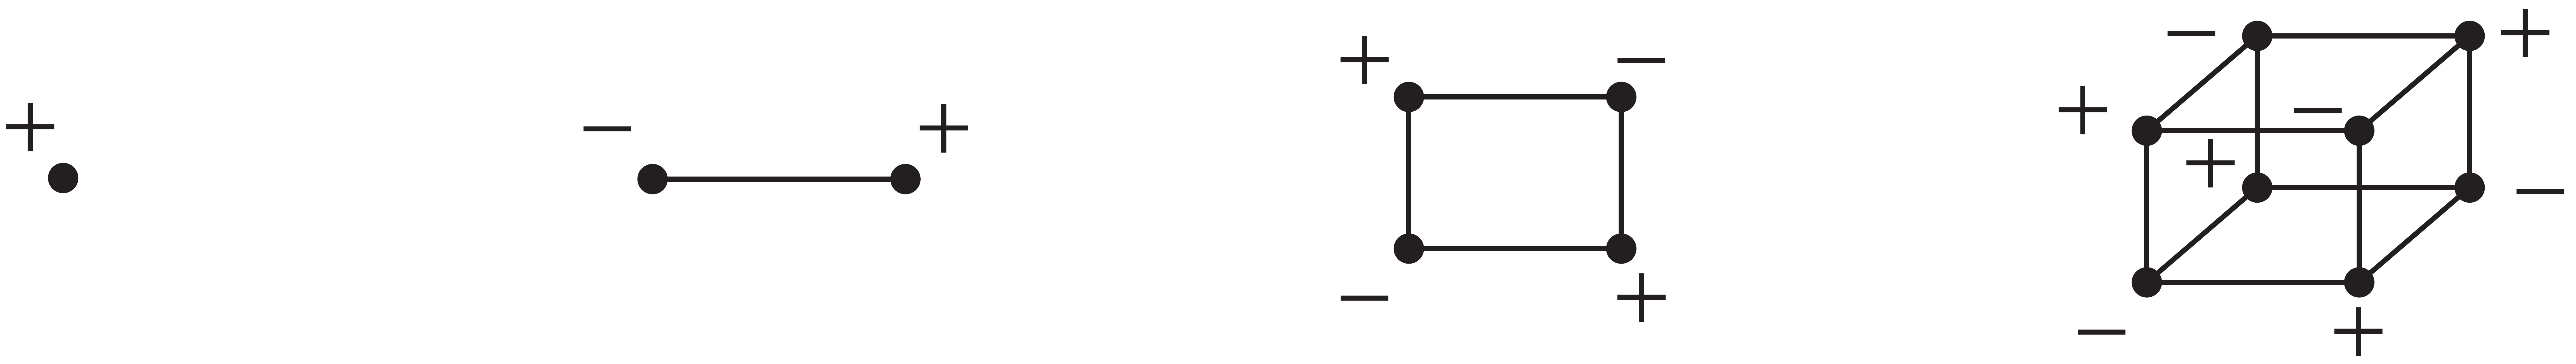
\includegraphics[width=\textwidth]{../Rss/Electromagnetism/Potential/MultiPoleHierarchy.png}
    \caption*{Monopole, Dipole, Quadrupole, and Octopole}
\end{figure*}

\subsubsection*{The Monopole and Dipole Terms.} Ordinarily, the multipole expansion is dominated (at large r) by the monopole
term:
\begin{equation*}
     V_{\text{mon}}(\mathbf{r})=\frac{1}{4\pi \epsilon_0}\frac{Q}{r},
\end{equation*}
where $\int\rho\; d\tau=Q$. For a point charge at the origin, $ V_{\text{mon}}$ is the exact potential, not merely a first approximation at large r; in this case, all the higher multipoles vanish. If the total charge is zero, the dominant term in the potential will be the dipole:
\begin{equation*}
     V_{\text{dip}}(\mathbf{r})=\frac{1}{4\pi \epsilon_0}\frac{1}{r^2}\int r'\cos \alpha \rho(\mathbf{r}')\; d\tau'.
\end{equation*}
Since $\alpha$ is the angle between $\mathbf{r'}$ and $\mathbf{r}$, then $r' \cos \alpha = \mathbf{\hat{r}} \cdot \mathbf{r'}$. Therefore, dipole potential can be written more succinctly:
\begin{equation*}
     V_{\text{dip}}(\mathbf{r})=\frac{1}{4\pi \epsilon_0}\frac{1}{r^2}\mathbf{\hat{r}}\cdot\int \mathbf{r'} \rho(\mathbf{r}')\; d\tau'.
\end{equation*}
This integral (which does not depend on r) is defined the dipole moment of the distribution
\begin{equation*}
    \mathbf{p}\equiv \int\mathbf{r'} \rho(\mathbf{r}')\; d\tau'.
\end{equation*}
Dipole contribution to the potential simplifies to
\begin{equation*}
     V_{\text{dip}}(\mathbf{r})=\frac{1}{4\pi \epsilon_0}\frac{\mathbf{p}\cdot \mathbf{\hat{r}}}{r^2}
\end{equation*}
Dipole moment translates in the usual way for point, line, and surface charges. Thus, the dipole moment of a collection of point charges is
\begin{equation*}
    \mathbf{p}=\sum_{i=1}^{n}q_i\mathbf{r'}_i
\end{equation*}
For a physical dipole (equal and opposite charges, $\pm q$),
\begin{equation*}
    \mathbf{p}=q\mathbf{r'}_+-q\mathbf{r'}_-=q\mathbf{d}
\end{equation*}
where \textbf{d} is the vector from the negative charge to the positive one. However, that this is only the approximate potential of the physical dipole--evidently there are higher multipole contributions. A physical dipole becomes a pure dipole, then, in the rather artificial limit $d \rightarrow0$, $q\rightarrow \infty$, with the product $qd = p$ held fixed. Dipole moments are vectors, and they add accordingly.

\subsubsection*{Origin of Coordinates in Multipole Expansions.} A point charge at the origin constitutes a “pure” monopole; if it is not at the origin, it's no longer a pure monopole. Point charge at \ref{fig:multipole1} has a dipole moment $\mathbf{p} = qd\; \mathbf{\hat{y}}$, and a corresponding dipole term in its potential. The monopole potential $(1/4\pi\epsilon_0)q/r$ is not quite correct for this configuration; rather, the exact potential is $(1/4\pi\epsilon_0)q/\rcurs$. The multipole expansion is a series in inverse powers of r (the distance to the origin), and when we expand $1/\rcurs$, we get all powers, not just the first.
\begin{figure}
    \centering
    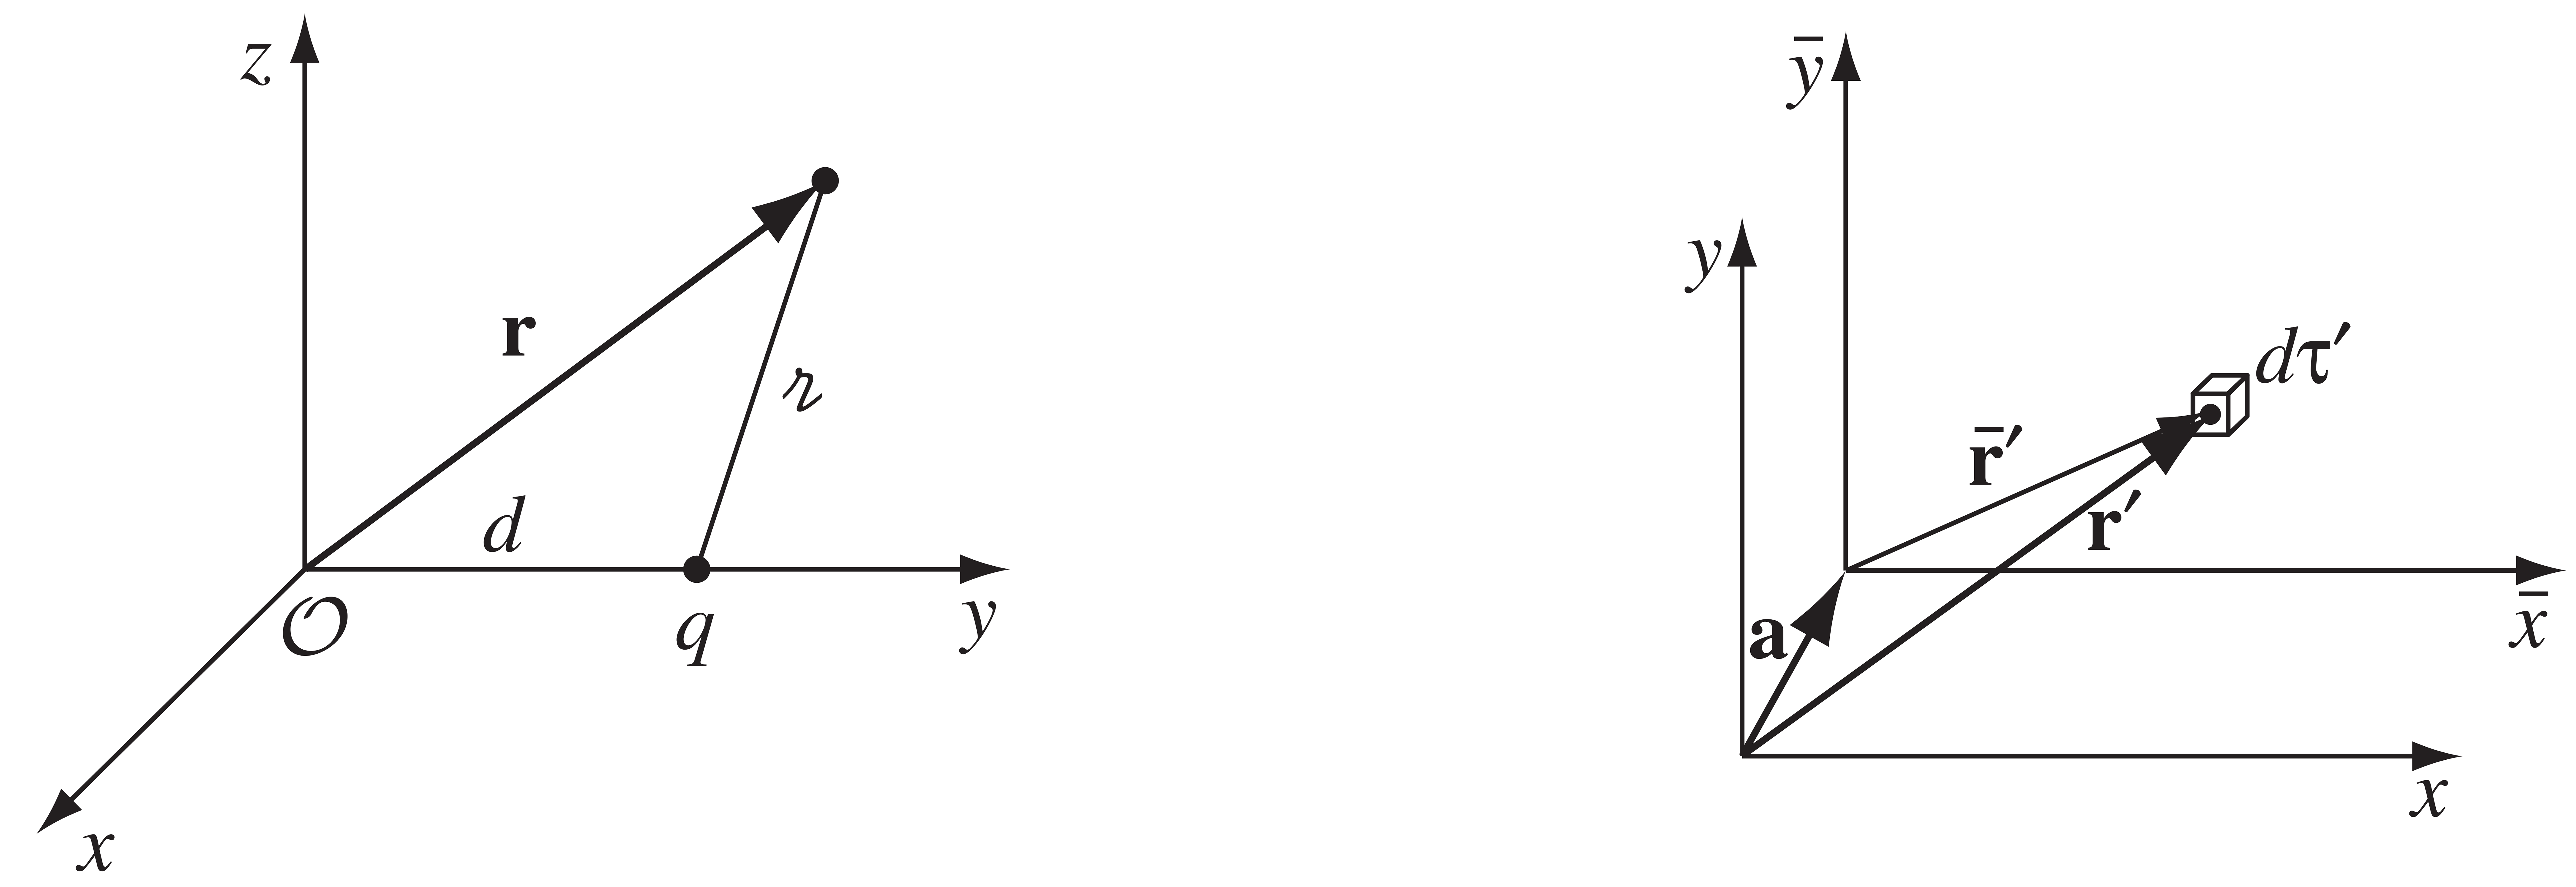
\includegraphics[width=\textwidth]{../Rss/Electromagnetism/Potential/MultipoleCoordinate.png}
    \caption{Point charge not at origin and point charge from different origin}
    \label{fig:multipole1}
\end{figure}

So moving the origin (or, what amounts to the same thing, moving the charge) can alter a multipole expansion. Ordinarily, the dipole moment does change when you shift the origin, but there is an important exception: If the total charge is zero, then the dipole moment is independent of the choice of origin.
\begin{align*}
    \mathbf{\bar{p}}&= \int\mathbf{\bar{r}'} \rho(\mathbf{r}')\; d\tau'\\
    &=\int(\mathbf{r'}-\mathbf{a}) \rho(\mathbf{r}')\; d\tau'\\
    &=\int\mathbf{r'} \rho(\mathbf{r}')\; d\tau'-\mathbf{a}\int \rho(\mathbf{r}')\; d\tau'\\
    &=\mathbf{p}-Q\mathbf{a}
\end{align*}

\subsubsection*{Electric Field of a Dipole.} If we choose coordinates so that $p$ is at the origin and points in the z direction, then the field at $ r, \theta$ is:
\begin{figure*}[h]
    \centering
    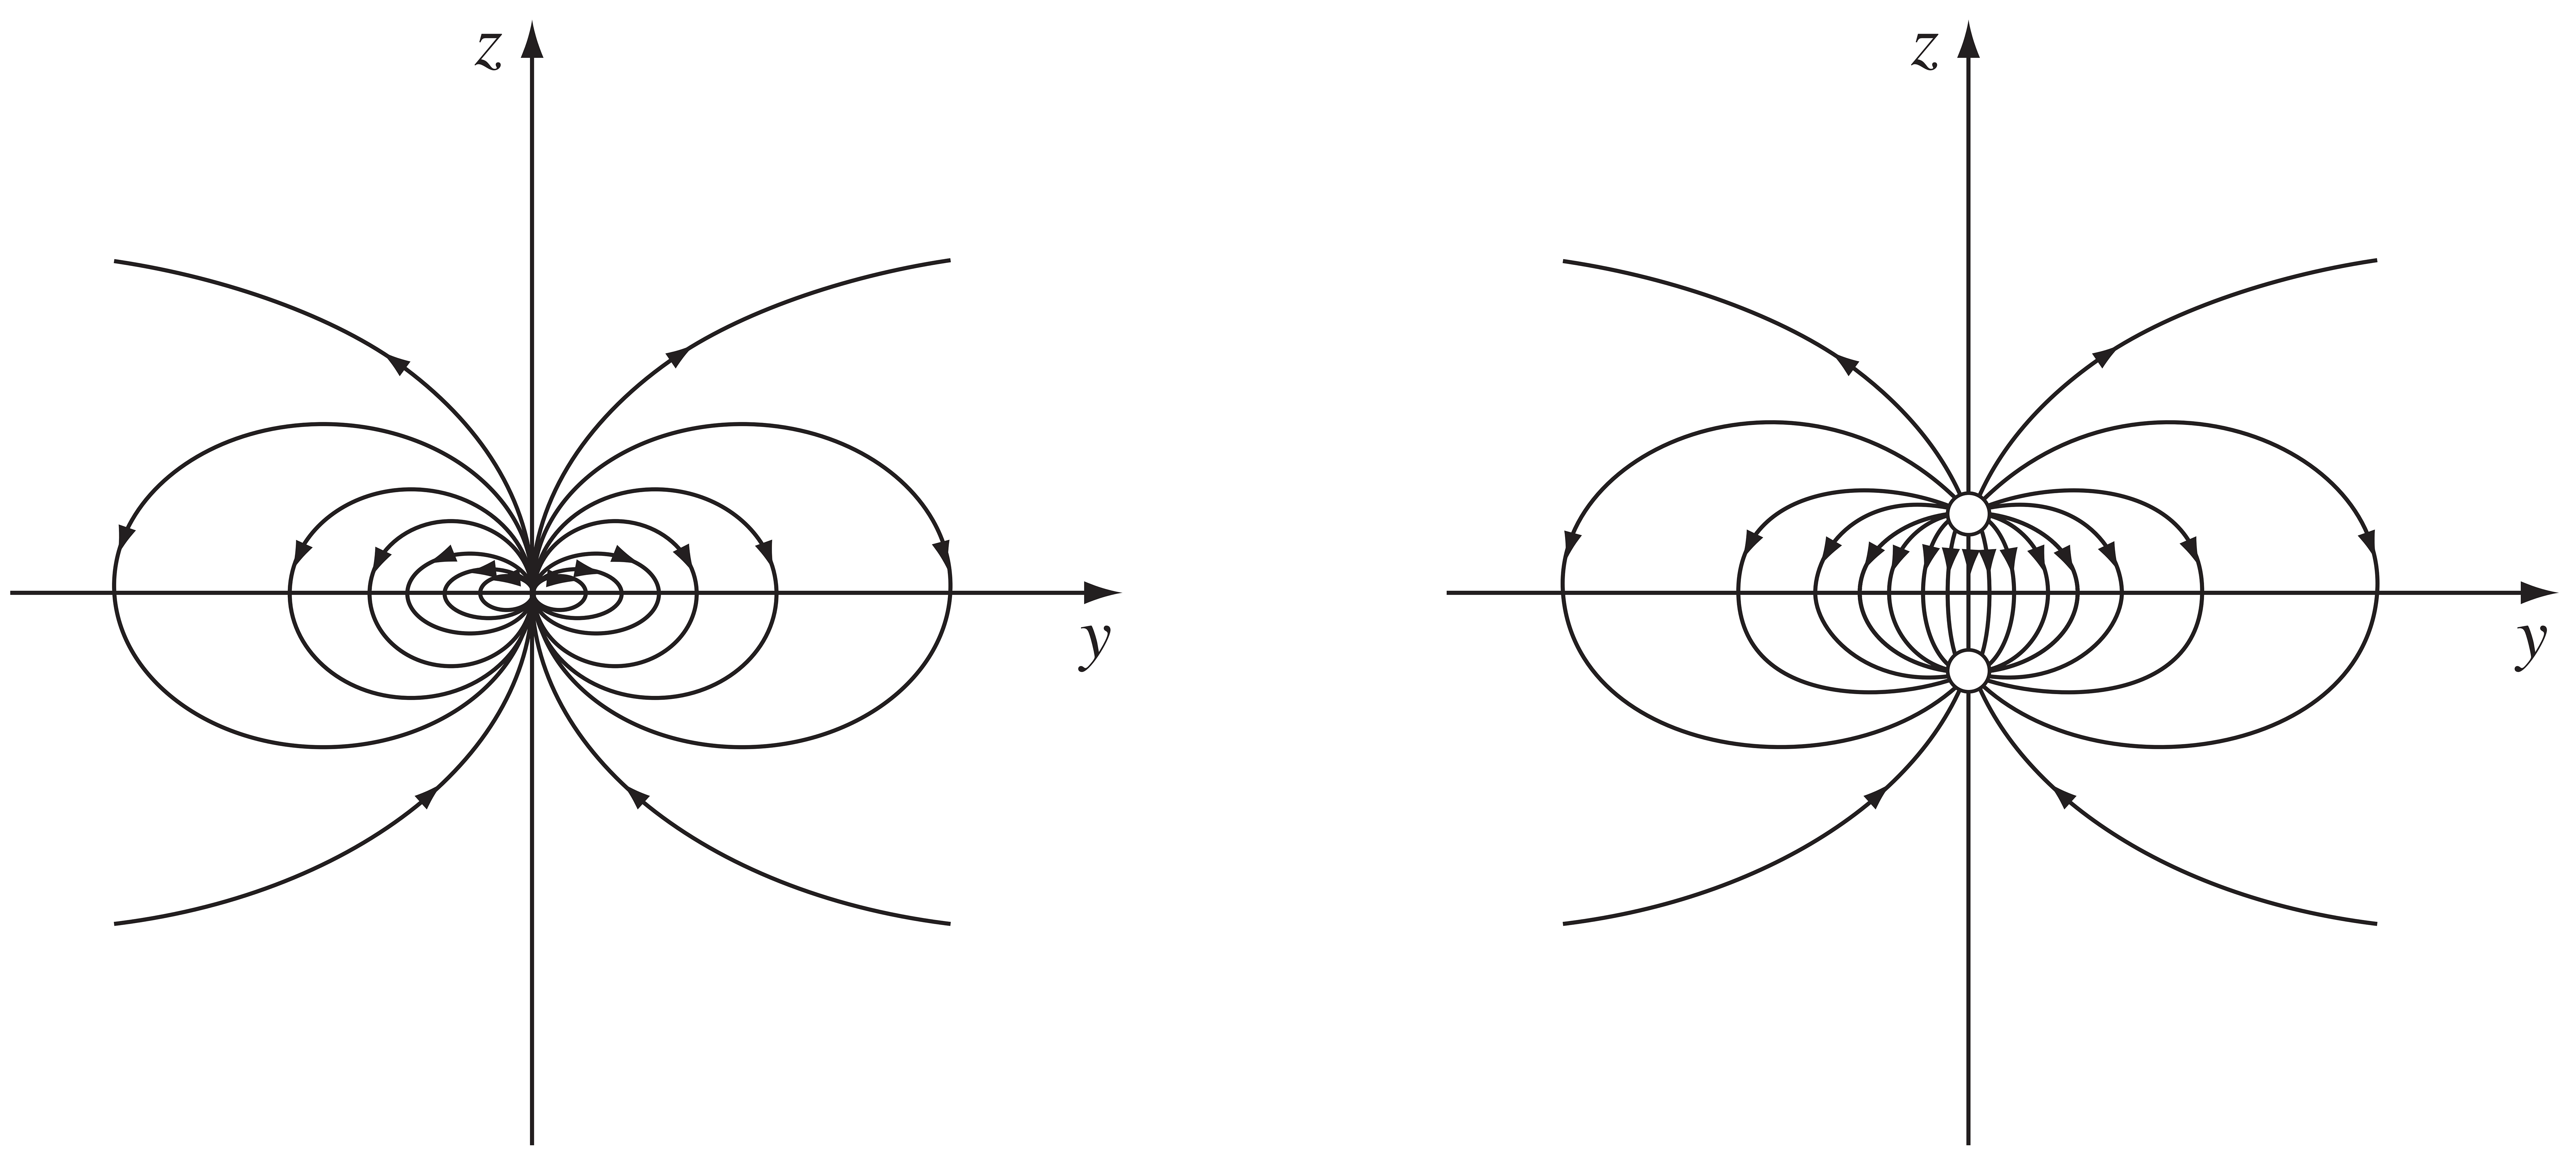
\includegraphics[width=\textwidth]{../Rss/Electromagnetism/Potential/MultiPoleField.png}
    \caption*{Figure: field of pure and real dipole}
\end{figure*}
\begin{equation*}
    \mathbf{E}_{\text{dip}}(r,\theta)=-\nabla V_{\text{dip}}(r,\theta)=\frac{p}{4\pi \epsilon_0r^3}(2\cos\theta\mathbf{\hat{r}}+\sin\theta\mathbf{\hat{\theta}})
\end{equation*}
This formula makes explicit reference to a particular coordinate system (spherical) and assumes a particular orientation for p (along z). Notice that the dipole field falls off as the inverse cube of r; the monopole field goes as the inverse square, of course. Quadrupole fields go like $1/r^4$, octopole like $1/r^5$, and so on.  

Notice how similar the fields become if you blot out the central region; up close, however, they are entirely different. Only for points $r >> d$ does $\mathbf{E}_{\text{dip}}$ represent a valid approximation to the field of a physical dipole. This régime can be reached either by going to large r or by squeezing the charges very close together.

\end{document}